\documentclass{IEEEtran}

\usepackage[left=1.5cm,right=1.5cm]{geometry}
\usepackage[
spanish,
es-nodecimaldot
%english
]{babel}
\usepackage[utf8]{inputenc}
\usepackage[T1]{fontenc}
\usepackage{float}
\usepackage{crossreftools}
\usepackage{graphicx}
\usepackage{grffile}
\usepackage{longtable}
\usepackage{wrapfig}
\usepackage{rotating}
\usepackage[normalem]{ulem}
\usepackage{amsmath}
\usepackage{textcomp}
\usepackage{amssymb}
\usepackage{capt-of}
\usepackage{hyperref}
\usepackage{minted}
\usepackage{subfiles}
\usepackage[acronym, toc]{glossaries}

\usepackage{fancyhdr}
\usepackage{graphicx}
\usepackage{xcolor}
\usepackage{multicol}

\usepackage{grffile}
\usepackage{longtable}
\usepackage{wrapfig}
\usepackage{rotating}
\usepackage[normalem]{ulem}
\usepackage{amsmath}
\usepackage{textcomp}
\usepackage{amssymb}
\usepackage{capt-of}
\usepackage{booktabs}
\usepackage{hyperref}
\usepackage{caption}

\definecolor{LightGray}{gray}{0.9}
\definecolor{DarkGray}{HTML}{191919}
\definecolor{custom}{HTML}{F8F8F8}

\newenvironment{code}{\captionsetup{type=listing}}{}

\usemintedstyle{emacs}

\usepackage[ruled,vlined]{algorithm2e}


\renewcommand{\listingscaption}{Código}
\renewcommand\listoflistingscaption{Índice de \listingscaption\@s}

\setminted[elixir]{frame=single,framesep=1mm,baselinestretch=0.5,breaklines=true,bgcolor=custom,fontsize=\scriptsize}
\setminted[shell-session]{frame=single,framesep=1mm,baselinestretch=0.5,breaklines=true,bgcolor=custom,fontsize=\scriptsize}
% \graphicspath{{./img_common}{./img}}
\usepackage[T1]{fontenc}
\renewcommand*\familydefault{\sfdefault} %% Only if the base font of the document is to be sans serif

% \pagestyle{fancy}
% \fancyfoot[R]{\thepage}
% \fancyfoot[C]{\includegraphics[width=0.05\textwidth]{inge_logo}}
% \fancyhead[L]{\leftmark}
% \fancyhead[R]{\rightmark}


\begin{document}
\title{Introducción al TFIDF}
\author{Romero Andrade Cristian}
\markboth{24~de~marzo~de~2021}{}
\maketitle{}
\tableofcontents{}

\section{Introducción}\label{sec:introduccion}
\IEEEPARstart{L}{a} medida Tf-idf  es una medida estadística que se utiliza
en la recuperación de información para evaluar la relevancia de los términos en
los documentos de una colección de documentos.

\begin{itemize}
  \item El tf-idf es el producto de dos estadísticas, frecuencia de término y frecuencia de documento inversa
        Hay varias formas de determinar los valores exactos de ambas estadísticas.
  \item Una fórmula que tiene como objetivo definir la importancia de una palabra clave o frase dentro de un documento o una página web.
\end{itemize}

\subsection{Frecuencia de término}\label{sec:frec-de-term}
La frecuencia del término, $tf(t, d)$, es la frecuencia del término $t$.
\[ tf(t,d)\frac{f_{t,d}}{\sum_{t^{i}\in d}f_{t^{i}, d}}\]
donde $f_{t, d}$ es el recuento bruto de un término en un documento, es decir,
el número de veces que el término $t$ aparece en el documento $d$.
Hay varias otras formas de definir la frecuencia de los términos:
\begin{itemize}
  \item el recuento bruto en sí mismo: $tf(t, d) = f(t, d)$.
  \item ``Frecuencias'' booleanas: $tf(t, d ) = 1$ si $t$ ocurre en $d$ y $0$ en caso
        contrario.
  \item frecuencia de término ajustada a la longitud del documento:
        $tf(t, d) = \frac{f_{t, d}}{(numero\ de\ palabras\ en\ d)}$.
  \item frecuencia escalada logarítmicamente: $tf(t, d) = \log{(1 + f_{ t , d})}$.
  \item frecuencia aumentada, para evitar un sesgo hacia documentos más largos,
        por ejemplo, frecuencia sin procesar dividida por la frecuencia sin
        procesar del término más frecuente en el documento.
        \[ tf(t,d)=0.5+0.5 \times \frac{f_{t, d}}{max\{f_{t^{i}, d}: t^{i} \in d\}} \]
\end{itemize}

\subsection{Frecuencia de documento inversa}\label{sec:frec-de-docum}
La frecuencia inversa del documento es una medida de cuánta información
proporciona la palabra, es decir, si es común o rara en todos los documentos.
Es la fracción inversa escalada logarítmicamente de los documentos que
contienen la palabra (obtenida dividiendo el número total de documentos
por el número de documentos que contienen el término, y luego tomando el
logaritmo de ese cociente):
\begin{itemize}
  \item $N$: Número total de documentos en el corpus $N = |D| $.
  \item $|\{d \in D : t \in d\}|$: número de documentos donde aparece el término,
        es decir, si el término no está en el corpus, esto dará lugar a una división por cero. Por lo tanto, es     común ajustar el denominador a $tf(t,d) \ne 01 + |\{d \in D : t \in d \}|$

\end{itemize}

\subsection{Frecuencia de término: frecuencia de documento inversa}\label{sec:frec-de-term-1}
Entonces tf – idf se calcula como:
\[ tf \times idf(t,d,D) = tf(t,d) \cdot idf(t,D)\]

\section{Desarrollo}\label{sec:desarrollo}

Para calcular la frecuencia de término (sección~\ref{sec:frec-de-term}) se
elimino los espacios, comas y palabras de poca utilidad para despues guradarlas
en una lista; para el manejo del lenguaje se convirtieron en átomos cada palabra.
\begin{code}
  \inputminted[firstline=5,lastline=26]{elixir}{../lib/corpus.ex}
\end{code}

Posteriormente obtemos la concurrencia de cada palabra (no se usa) en el texto,
e inmediatamente se separa la palabras en listas de diez dentro de una lista.
\begin{code}
  \inputminted[firstline=29,lastline=43]{elixir}{../lib/corpus.ex}
\end{code}

Se calcula $idf$ usando la formula del logaritmo planteada en las
sección~\ref{sec:frec-de-docum}:
\begin{code}
  \inputminted[firstline=45,lastline=49]{elixir}{../lib/corpus.ex}
\end{code}

Se calcula $tf$ usando la formula del  el recuento bruto en sí mismo
planteada en las
sección~\ref{sec:frec-de-term}:
\begin{code}
  \inputminted[firstline=51,lastline=56]{elixir}{../lib/corpus.ex}
\end{code}

y para frecuencia de término: frecuencia de documento inversa:
\begin{code}
  \inputminted[firstline=65,lastline=67]{elixir}{../lib/corpus.ex}
\end{code}

Para obtener la gráficas se uso una biblioteca que usa ploty.js para renderizarla
en un documento html (figura~\ref{fig:1}).
\\\\\\\\\\\\
\begin{figure}[h!]
  \centering
  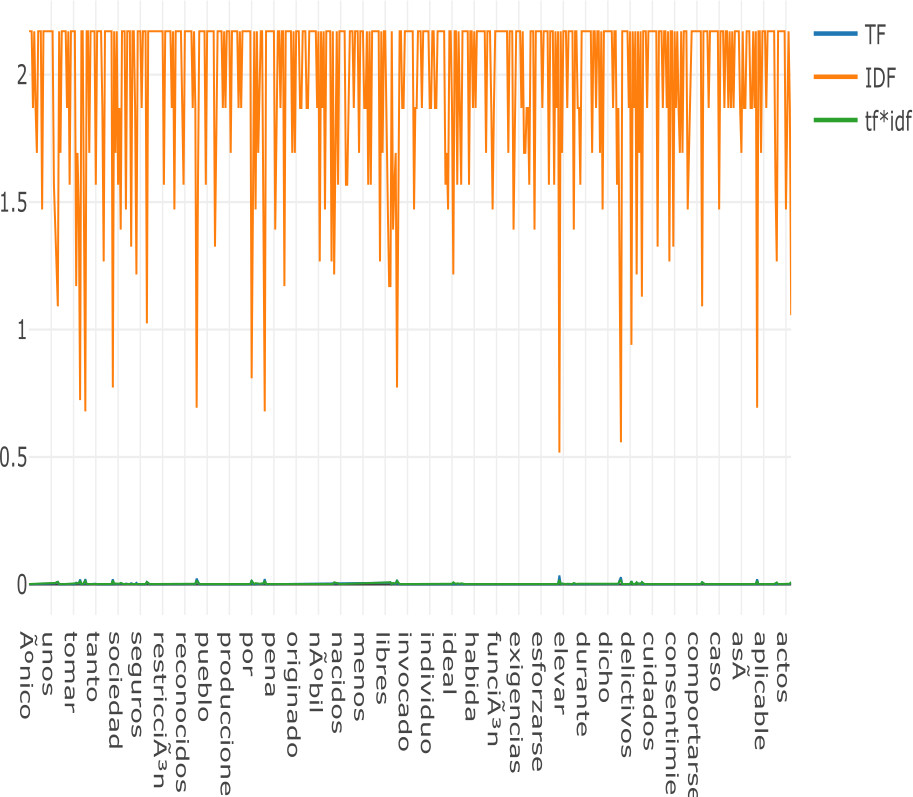
\includegraphics[width=\linewidth]{./output}
  \caption{Dercarga de svg generada por el doc html generado}\label{fig:1}
\end{figure}

También se genera un archivo CSV para comparar resultados.
\begin{table}[H]
  \centering{}
  \begin{tabular}{|l|l|l|l|}
    \hline
    Palabra  & TF                & IDF              & TDxIDF            \\ \hline
    �nico    & 0.000677 & 2.170261 & 0.00147 \\ \hline
    �ndole   & 0.000677 & 2.170261 & 0.00147 \\ \hline
    �tnicos  & 0.000677 & 2.170261 & 0.00147 \\ \hline
    �l       & 0.001355  & 1.869231 & 0.00253 \\ \hline
    y        & 0.000677 & 2.170261 & 0.00147 \\ \hline
    voto     & 0.001355  & 1.869231 & 0.00253 \\ \hline
    voluntad & 0.002033 & 1.693140  & 0.00344 \\ \hline
    vivienda & 0.000677 & 2.170261 & 0.00147 \\ \hline
    viudez   & 0.000677 & 2.170261 & 0.00147 \\ \hline
    violen   & 0.000677 & 2.170261 & 0.00147 \\ \hline
    \ldots   & \ldots & \ldots & \ldots \\ \hline
  \end{tabular}



\end{table}

\section{Compilación y ejecución}\label{sec:compilacion}

Usando un sistema arch linux,
mediante el uso del gestor de paquetes ejecutar los siguientes
comandos(como administrador) para instalar elixir, donde tambien instalará
la máquina virtual de erlang.

\begin{minted}{shell-session}
# pacman -S elixir
\end{minted}

Clonamos el repositorio \url{https://github.com/tysyak/corpus.git}, obtenemos las
dependencias y lo compilamos para generar el ejecutable para despues
ejecutarlo como argumento el texto.
\begin{minted}{shell-session}
sh-5.1$ git clone https://github.com/tysyak/corpus.git
Clonando en 'corpus'...
remote: Enumerating objects: 30, done.
remote: Counting objects: 100% (30/30), done.
remote: Compressing objects: 100% (20/20), done.
remote: Total 30 (delta 6), reused 30 (delta 6), pack-reused 0
Recibiendo objetos: 100% (30/30), 1.09 MiB | 2.57 MiB/s, listo.
Resolviendo deltas: 100% (6/6), listo.
sh-5.1$ cd corpus/
sh-5.1$ mix deps.get
* Getting plotly_ex (https://github.com/tysyak/plotly_ex.git)
remote: Enumerating objects: 8, done.
remote: Counting objects: 100% (8/8), done.
remote: Compressing objects: 100% (7/7), done.
remote: Total 135 (delta 0), reused 6 (delta 0), pack-reused 127
Resolving Hex dependencies...
Dependency resolution completed:
Unchanged:
  jason 1.2.2
* Getting jason (Hex package)
sh-5.1$ mix escript.build
==> jason
Compiling 8 files (.ex)
Generated jason app
==> plotly_ex
Compiling 2 files (.ex)
Generated plotly_ex app
==> corpus
Compiling 1 file (.ex)
Generated corpus app
Generated escript corpus with MIX_ENV=dev
sh-5.1$ ./corpus textos/es.txt
listening on http://localhost:39715
accepted. quitting...
listening on http://localhost:44845
accepted. quitting...
listening on http://localhost:33977
accepted. quitting...
listening on http://localhost:46283
accepted. quitting...
\end{minted}


\end{document}
